%%%%%%%%%%%%%%%%%%%%%%% file template.tex %%%%%%%%%%%%%%%%%%%%%%%%%
%
% This is a general template file for the LaTeX package SVJour3
% for Springer journals.          Springer Heidelberg 2010/09/16
%
% Copy it to a new file with a new name and use it as the basis
% for your article. Delete % signs as needed.
%
% This template includes a few options for different layouts and
% content for various journals. Please consult a previous issue of
% your journal as needed.
%
%%%%%%%%%%%%%%%%%%%%%%%%%%%%%%%%%%%%%%%%%%%%%%%%%%%%%%%%%%%%%%%%%%%
%
% First comes an example EPS file -- just ignore it and
% proceed on the \documentclass line
% your LaTeX will extract the file if required
\begin{filecontents*}{example.eps}
%!PS-Adobe-3.0 EPSF-3.0
%%BoundingBox: 19 19 221 221
%%CreationDate: Mon Sep 29 1997
%%Creator: programmed by hand (JK)
%%EndComments
gsave
newpath
  20 20 moveto
  20 220 lineto
  220 220 lineto
  220 20 lineto
closepath
2 setlinewidth
gsave
  .4 setgray fill
grestore
stroke
grestorew
\end{filecontents*}
%
\RequirePackage{fix-cm}
%
%\documentclass{svjour3}                     % onecolumn (standard format)
%\documentclass[smallcondensed]{svjour3}     % onecolumn (ditto)
\documentclass[smallextended]{svjour3}       % onecolumn (second format)
%\documentclass[twocolumn]{svjour3}          % twocolumn
%
\smartqed  % flush right qed marks, e.g. at end of proof
%
\usepackage{graphicx}
\usepackage{xcolor}
\usepackage{listings}
%
% \usepackage{mathptmx}      % use Times fonts if available on your TeX system
%
% insert here the call for the packages your document requires
%\usepackage{latexsym}
% etc.
%
% please place your own definitions here and don't use \def but
% \newcommand{}{}
%
% Insert the name of "your journal" with
% \journalname{myjournal}
%
\begin{document}

\title{Citation Analysis of Computer Science Publications}
%\thanks{Grants or other notes
%about the article that should go on the front page should be
%placed here. General acknowledgments should be placed at the end of the article.}

\subtitle{Relationship To Other Fields}

%\titlerunning{Short form of title}        % if too long for running head

\author{Sitaram Devarakonda  \and
	Dmitriy Korobskiy \and
        Tandy Warnow \and
        George Chacko }

%\authorrunning{Short form of author list} % if too long for running head

\institute{Sitaram Devarakonda,  \at
              Netelabs, NET ESolutions Corporation, McLean, VA \\
              %Tel.: +123-45-678910\\
              %Fax: +123-45-678910\\
              \email{sitaram@nete.com}           %  \\
%             \emph{Present address:} of F. Author  %  if needed
           \and
              Dmitriy Korobskiy \at
              Netelabs, NET ESolutions Corporation, McLean, VA  \\
              \email{dk@nete.com}
           \and
           Tandy Warnow \at
              Dept of Computer Science, University of Iliinois Urbana-Champaign, Champaign IL \\
              \email{warnow@illinois.edu}
           \and
           George Chacko \at
              Netelabs, NET ESolutions Corporation, McLean, VA \\
              \email{netelabs@nete.com}
}

\date{Received: date / Accepted: date}
% The correct dates will be entered by the editor

\maketitle

\begin{abstract}
Computer science as a field has experienced dramatic growth and diversification over the last twenty years. Towards an improved understanding of the structure of the field, we analyze a cohort of the computer science literature.  For insight on the features of this cohort and the flow of information within its components, we construct article level clusters whose elements are linked by citations or co-citations, and reconcile them with major and minor subject categories in the All Science Journal Classification (Scopus). [abstract is feeble and needs to be rewritten]

\keywords{Bibliometrics \and Clustering \and Research Evaluation \and Computer Science}
% \PACS{PACS code1 \and PACS code2 \and more}
\subclass{01A85 \and 01A90} %\and more}

\end{abstract}

\section{Introduction}
\label{intro}

Computer science, and its applications, has experienced rapid growth and diversification over the last twenty years. More recently, the collective influence of the Internet of Things (IoT), `big' data, accessible cloud computing, and advances in artificial intelligence have been postulated as a recent driver for growth and evolution~\cite{siebel2019_digital}. As noted in a 2017 US National Academies Report~\cite{nas_2017}, ``A wide range of jobs in virtually all sectors demand computing skills to an unprecedented extent. And every academic discipline finds itself incorporating computing into its research and educational mission". Given this powerful influence some understanding of the present state and structure of computer science and its relationship to other fields would inform planning and policy making at multiple levels from national level funding all the way down to faculty hiring strategy. For the same reason of broad influence, computer science can also serve as a model system for studying interdisciplinarity. 

Noting that that the scientific literature serves a rich source of information to study the structure and historical development of a field, Salton and Bergmark conducted a historical study  of the computer science literature (419 computer articles published in 1974,  and 3,812 references cited in these articles)~\cite{salton_citation_1979}. These authors described the global structure of computer science as comprising three main subareas (i) theoretical foundations, such as theory of computation, (ii) hardware and computer systems, such as architecture,  and (iii) software, such as programming systems.  Related areas noted were (a) mathematics of computing, such as numerical analysis, (b) special software topics, such as operating systems, (c) data management and database systems, (d) methodologies valid for multiple applications, such as algebraic manipulation, (e) computer applications, such as computer graphics, (f) non-technical aspects, such as computer education. 

Computing has grown and evolved significantly since 1974. Progressing beyond Salton and Bergmark's historical triad of theoretical foundations; hardware and computer systems; and software, the Computing Classification System (CCS)~\cite{acm_ref} published by the Association for Computing Machinery now consists of 13 top-level areas that reflect a more current view of the field. This classification also addresses relationships with other fields under the category of Applied Computing. However, an easy way to map scientific publications, especially interdisciplinary articles or those from adjacent fields, to the CCS classification does not exist. 

Other classification systems are available such as the All Science Journal Classification (ASJC) developed and maintained by Scopus. the Web of Science research and categorical classifications from Clarivate Analytics, and the NSF classification system~\cite{nsf_classification}. Of these, Scopus and the Web of Science also include global bibliographies with citation links and proprietary unique identifiers for publications that can be matched, in some cases, to digital object identifiers (DOIs). All three rely on applying one or more journal-derived labels to articles. The inheritance, by articles, of labels meant to describe journals can be problematic in fields that evolve faster than their journal classifications. Shu and colleagues recently noted in a comparative study of the Chinese Science Citation Database (CSCD) and the Web of Science, that 46\% of articles did not belong to the discipline of the journal they were published in~\cite{shu_comparing_2019}. Others have also discussed and critiqued disciplinary assignments using journal based classifications~\cite{wang_large-scale_2016} \textcolor{blue}{need comprehensive list of citations}. Article classification systems have been constructed, however, which escape some of the criticisms of journal-based classification~\cite{traag_louvain_2019,boyack_classification_2014,waltman_new_2012}.
  
In this study, we sought to extend the work of Salton and Bergmark to reflect a more current reality while also considering connections between computer science and other fields. As a source of computer science literature, we used DBLP, a reference bibliography for computer science~\cite{dblp_ref}. The DBLP bibliography covers publications from computer science and includes publications from hybrid fields, where they are considered pertinent to computer science research. The underlying assumption is that records in DBLP are greatly enriched for computer science even while recognizing that coverage may be incomplete and possibly biased. Cross-matching DBLP publications to Scopus records enabled us to harvest the richer citation data in Scopus, as well as extract links to publications from other disciplines. This cross-matching also allows the use of both journal and article based classifications when clustering documents. Using both direct citations and co-citations as the basis for clustering, we used DBLP articles from journals and conference proceedings for the period 1996-2015. We reconciled these clusters with the All Science Journal Classification (ASJC) developed and maintained by Scopus through a combination of automated and manual procedures. We describe below the high-level interactions of computer science within the Physical Sciences as well as with the Social Sciences and Life Sciences. 

\section{Materials and Methods}
\label{sec:methods}

\subsection{Data}
 A stable release of the DBLP computer science bibliography~\cite{dblp_ref} consisting of 7,079,994 records was downloaded as dblp-2018-08-01.xml.gz. Publications were parsed from the xml source file and loaded into a PostgreSQL database. We have previously parsed, the Scopus dataset of over 72,000,000 publications into a custom schema as part of a larger data platform for research evaluation~\cite{GithubERNIE2019}. Records in the DBLP dataset, were matched to Scopus identifiers using digital object identifiers (DOIs). This procedure resulted in a dataset of 2,685,356 DBLP publications with Scopus identifiers where 1,278,322 (47.6\%) were labeled as article and 1,407,034 (52.4\%) as conference proceedings. References cited by these publications were then extracted from Scopus (7,129,006), resulting in a total of 8,000,411 nodes (publications and references) and  44,296,381 edges that represent citations within the dataset. This dataset is referred to as \emph{comp} (see Fig~\ref{fig:ar_cp_annotation}).
 
 \begin{figure}[ht]
\centering
% Use the relevant command to insert your figure file.
% For example, with the graphicx package use
  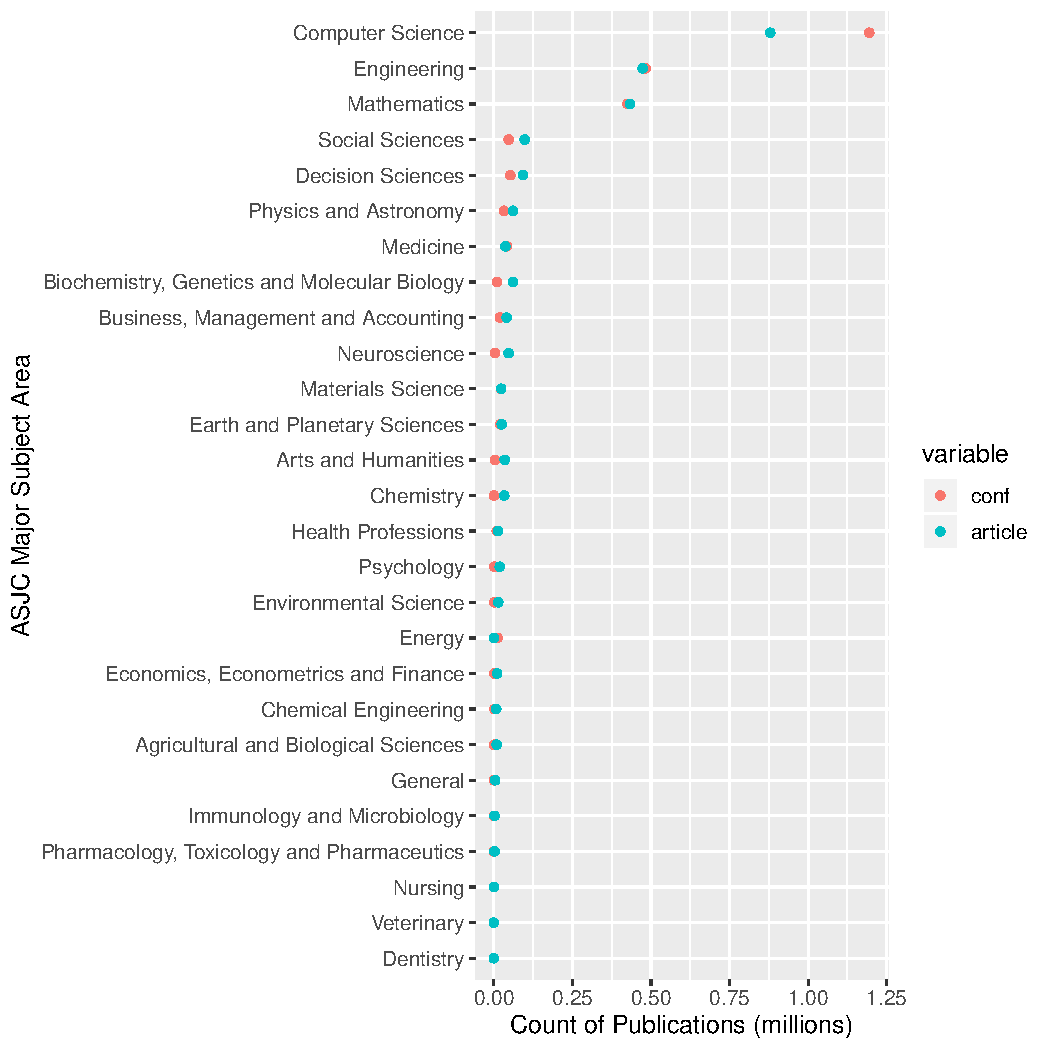
\includegraphics[scale=0.5]{ar_cp_ratio.pdf}
% figure caption is below the figure
\caption{Summary of DBLP data cross-matched with Scopus. 2,685,356 publications from DBLP were cross-matched with Scopus and then grouped by the 27 major subject areas in the ASJC (Scopus) classification. The largest number of publications are contributed by Computer Science; Mathematics; and Engineering and then by Social Sciences; Physics and Astronomy; and Biochemistry, Genetics, and Molecular Biology. Publications were further annotated with respect to being either articles \emph{(ar)} or conference proceedings \emph{(cp)}. For this dataset, the major subject areas of Computer Science (2,059,120 (cp), 1,576,691 (ar); Engineering; and Mathematics contributed the most publications while Pharmacology, Toxicology, and Pharmaceutics; Nursing, Veterinary and Dentistry (1 ar) contributed the least.}
\label{fig:ar_cp_annotation}       % Give a unique label
\end{figure}

\subsection{Clustering methods}

\paragraph{Clustering by Direct Citation} Graclus is a spectral graph clustering package that computes normalized cut and ratio association for a given undirected graph~\cite{graclus_2007}.  We used v1.2 in our experiments. The \emph{comp} dataset was formatted as an undirected graph, stored in a file with a header line indicating the number of nodes and edges, and used as input to Graclus, which requires the number of clusters to be formed as an input parameter. In preliminary experiments, we varied the number of clusters to be formed between 10 and 50 clusters (data not shown).  At 20 clusters, the most evenly sized set of clusters resulted with the largest cluster containing roughly 10 times the number of nodes in the smallest one~\cite{traag_louvain_2019}.  Consequently, we generated 20 clusters, labeled 0-19, using Graclus (Fig~\ref{fig:heatmap}). The quality of clustering was evaluated by measuring conductance as defined in Shun et al.~\cite{shun_parallel_2016}. Data in \emph{comp} were clustered into 18, 20, or 22 clusters and in each case the highest numbered cluster (17, 19, or 21) had the greatest conductance value and the smallest number of nodes suggesting that it effectively served as a container for `left over publications' during the Graclus process. Thus, we did not consider cluster 19 (the 20th cluster) when interpreting our results.  The remaining 19 clusters had conductance values ranging from 0.09 to 0.25 with a median conductance of 0.15.

 \begin{figure}[ht]
\centering
% Use the relevant command to insert your figure file.
% For example, with the graphicx package use
  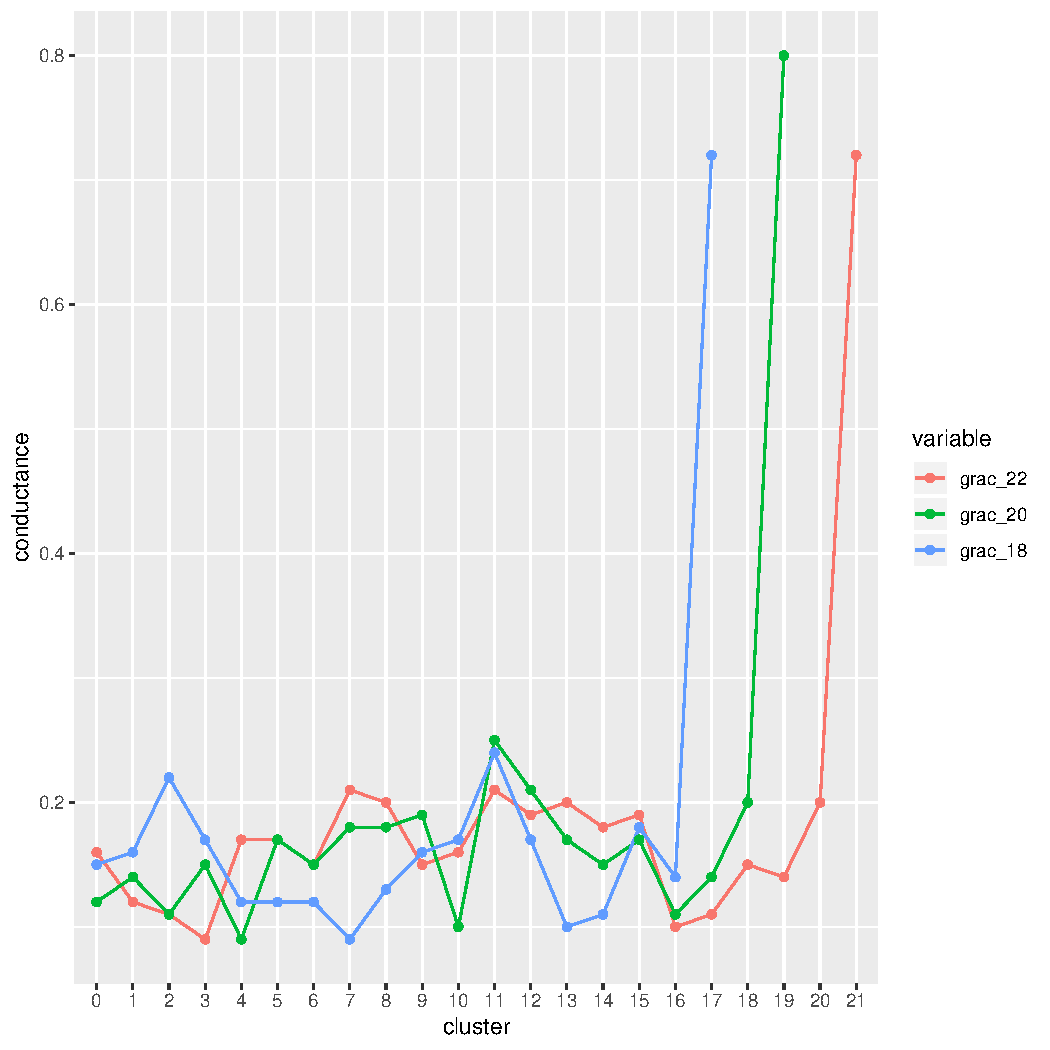
\includegraphics[scale=0.3]{graclus_comparison.pdf}
% figure caption is below the figure
\caption{Summary of DBLP data cross-matched with Scopus. 2,685,356 publications from DBLP were cross-matched with Scopus and then grouped by the 27 major subject areas in the ASJC (Scopus) classification. The largest number of publications are contributed by Computer Science; Mathematics; and Engineering and then by Social Sciences; Physics and Astronomy; and Biochemistry, Genetics, and Molecular Biology. Publications were further annotated with respect to being either articles \emph{(ar)} or conference proceedings \emph{(cp)}. For this dataset, the major subject areas of Computer Science; Engineering; and Mathematics contributed the most publications while Pharmacology, Toxicology, and Pharmaceutics; Nursing, Veterinary and Dentistry contributed the least.}
\label{fig:graclus_comparison}       % Give a unique label
\end{figure}


\begin{table}
% table caption is above the table
\caption{\emph{2685021 is because of inner joins on ASJC Explain conductance calculations~\cite{shun_parallel_2016}}}
\label{tab:1}       % Give a unique label
% For LaTeX tables use
\begin{tabular}{lllll}
\hline\noalign{\smallskip}
Cluster & Publications & Conductance & Total ASJC Labels & Unique ASJC Labels\\
\noalign{\smallskip}\hline\noalign{\smallskip}
0 & 111,294 & 0.12 & 265,664 & 142 \\ 
1 & 117,057 & 0.14 & 246,960 & 166 \\ 
2 & 116,251 & 0.11 & 280,602 & 165 \\ 
3 & 353,366 & 0.15 & 881,693 & 200 \\ 
4 & 145,081 & 0.09 & 349,020 & 154 \\ 
5 & 92,097 & 0.17 & 248,168 & 186 \\ 
6 & 71,865 & 0.15 & 199,681 & 163 \\ 
7 & 179,927 & 0.18 & 465,181 & 202 \\ 
8 & 302,656 & 0.18 & 760,117 & 214 \\ 
9 & 69,520 & 0.19 & 197,031 & 174 \\ 
10 & 42,462 & 0.10 & 102,838 & 141 \\ 
11 & 448,030 & 0.25 & 1,229,061 & 224 \\ 
12 & 70,738 & 0.21 & 216,546 & 179 \\ 
13 & 105,232 & 0.17 & 289,318 & 187 \\ 
14 & 199,176 & 0.15 & 551,657 & 208 \\ 
15 & 64,384 & 0.17 & 195,679 & 167 \\ 
16 & 89,340 & 0.11 & 240,157 & 158 \\ 
17 & 50,817 & 0.14 & 181,531 & 179 \\ 
18 & 43,113 & 0.20 & 108,518 & 177 \\ 
19 & 12,615 & 0.80 & 36,583 & 229 \\ \noalign{\smallskip}\hline
\end{tabular}
\end{table}

\paragraph{Clustering by Co-Citation} To build clusters using co-citations, we first implemented variable level clustering, an approach developed by Small and Sweeney (1985)~\cite{small_clustering_1985}, with minor modifications. Variable level clustering involves applying a threshold (below which all edges in a graph are dissolved) then iteratively selecting edges with the highest normalized co-citation value and extracting connected components from the graph as clusters for each edge in turn. Three parameters are needed (i) a threshold or starting level based on a quantile of normalized co-citation frequency (ii) a level increment (iii) a maximum cluster size. An issue is the generation of very large clusters by chaining through low edge weights.  Thus, at each iteration, any cluster exceeding the maximum cluster size returned to the process and a higher threshold applied to break such clusters.

In our implementation of variable level clustering, we first calculated the number of citations accumulated across Scopus for all 2,685,356 articles in \emph{comp}. After discarding those publications without any citations, \textcolor{blue}{Sitaram please confirm}, we restricted further analysis to those in the 90th percentile of citations or higher resulting in a dataset of size 212,311. We then identified 4,318,305 publications in Scopus that cite these 212,311 articles from \emph{comp}. For each of the 4,318,305 citing publications in turn, all possible reference pairs, ${n \choose 2}$, were generated where $n$ is the number of references in a publication. The cited reference pairs were restricted to those in the set of 212,311 highly cited papers previously identified.The frequency of these co-cited pairs was then computed across the dataset  and normalized using Salton's cosine formula~\cite{salton_citation_1979}. A total of 46,463,117 unique co-cited pairs were thus obtained. These data were represented in a graph where each node was a publication and the weighted edge between the pair was the normalized co-citation frequency. \par

We applied variable clustering with initial parameters of threshold ($t$) = median normalized co-citation frequency (quantile=0.5), increment $i = 0.1$, and maximum cluster size, $mcs=200$. Thus, at start, all edges below the median normalized co-citation frequency are dissolved. Clusters were formed by assembling connected components from each co-cited pair beginning with the heaviest edge weight. Clusters below size 100 were retained and any cluster larger than 200 nodes was carried over to the next round. The threshold, $t$, was then incremented by 0.1 and the process repeated while progressively incrementing $t$.  We used a bi-phasic approach where in which $t$ ranged from 0.5-0.9, after which $i$ was reduced to 0.01 for the range $0.9 \leq t \leq 0.99$. A final threshold of $t$=0.999 was applied to break the single remaining large cluster. All clusters generated thus, contained  less than 100 nodes.  Using this approach, 22,232 clusters containing 84,591 nodes were generated. Clusters containing only 2 nodes were then discarded bringing the total number of clusters down to 10,298. 

Agglomerative clustering was then performed on these 10,298 clusters to generate higher-order clusters. Briefly, each cluster was now treated as a node and the edge weight between two clusters was assigned as the maximum edge weight of all edges between the nodes in these two clusters. Edges were arranged in descending order. The first pair of clusters were merged and its edge weight with other interacting clusters was recalculated. All edges were then re-ordered as before and the next pair of clusters was merged. The process was halted after 600 rounds to prevent single large clusters being generated (figure).

\begin{figure}[ht]
% Use the relevant command to insert your figure file.
% For example, with the graphicx package use
  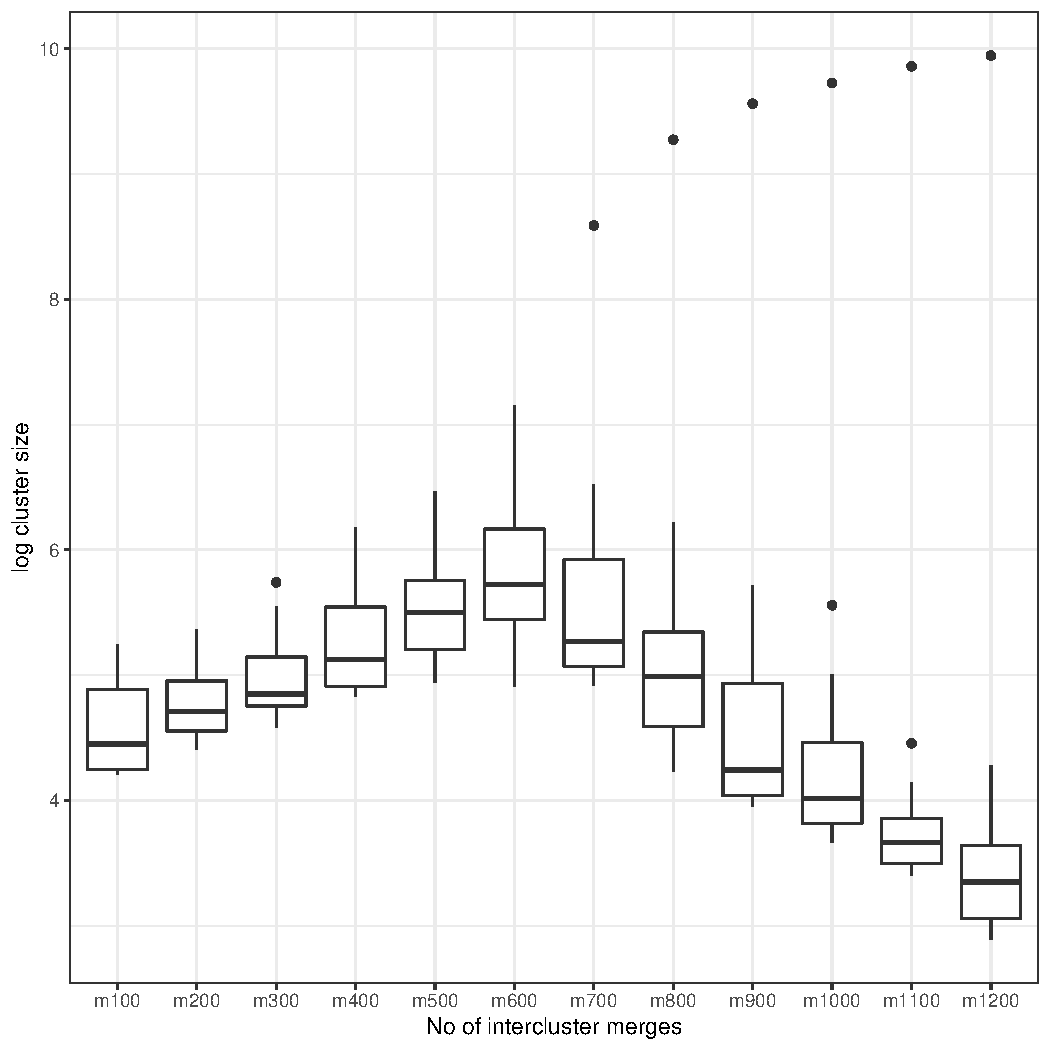
\includegraphics[scale=0.5]{merge_select.pdf}
% figure caption is below the figure
\caption{caption will be inserted I just haven't been able to overcome the threshold to avoid boring tasks}
\label{fig:merge_select}       % Give a unique label
\end{figure}

\section{Results}
\label{sec:results}

\begin{figure}[ht]
% Use the relevant command to insert your figure file.
% For example, with the graphicx package use
  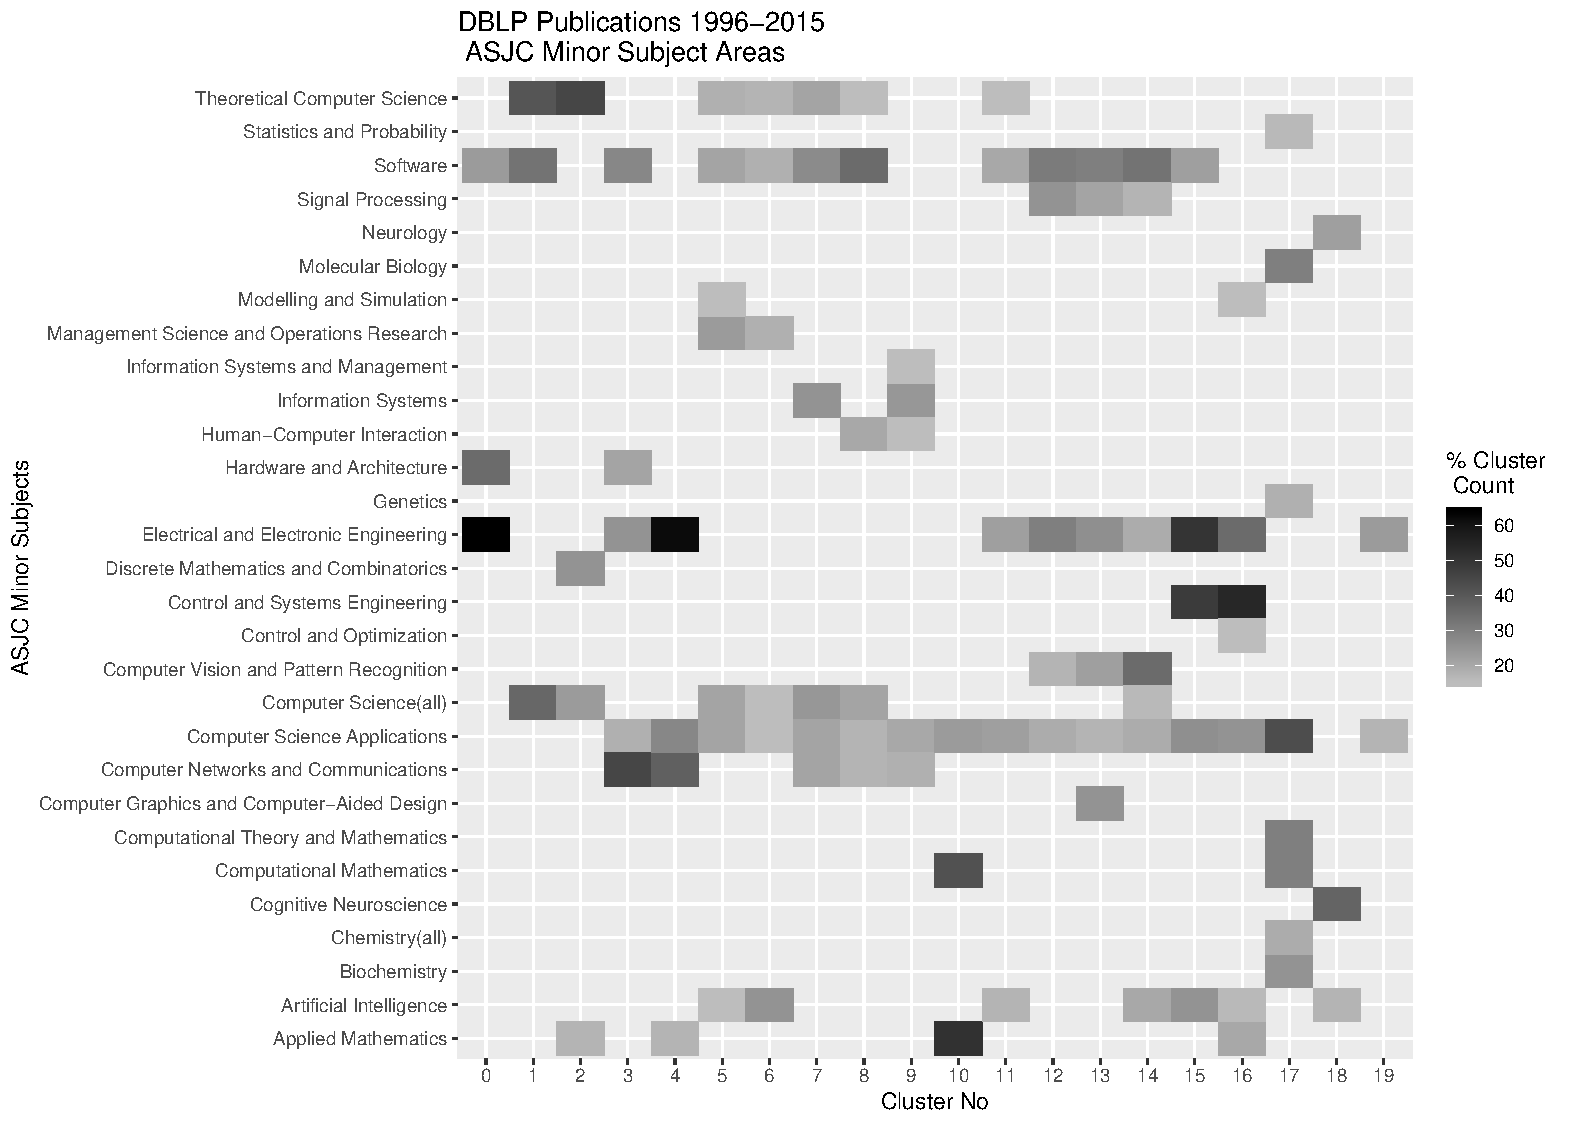
\includegraphics[scale=0.5]{scopus_dblp_graclus3.pdf}
% figure caption is below the figure
\caption{caption will be inserted I just haven't been able to overcome the threshold to avoid boring tasks}
\label{fig:heatmap}       % Give a unique label
\end{figure}

For the purpose of this study, our working definition of the computer science literature was all publications in the DBLP bibliography published in the years 1996-2015, that had (i) a digital object identifier (DOI), and (ii) could also be matched to article identifiers in the Scopus bibliography. The process of selection and matching resulted in a dataset of 2,685,356 publications (Materials and Methods). 

\emph{Clustering by Direct Citation.} Clustering of publications is commonly accomplished through direct citation, bibliographic coupling, and co-citation with an argument being made for direct citation as the best approach to concentrate citation links~\cite{klavans_which_2017}. Accordingly, we first used direct citation links as the basis for cluster formation. A set of 20 clusters was generated using Graclus, a spectral clustering technique that has previously been applied to citation data~\cite{graclus_2007,subelj_clustering_2016}. Considering the caveats associated with generating \emph{comp}, namely, the coverage limitations of the DBLP dataset (ii) cross-matching to Scopus (iii) journal based classification (iv) clustering, we constructed article level clusters of this computer science dataset at a sufficiently high level of aggregation to avoid cognitive challenge and cross-matched them to disciplinary classification by journal, the Scopus ASJC classification. We only considered Scopus ASJC minor subject area categories that accounted for at least 10\% of the publications in each cluster. 

(Fig~\ref{fig:heatmap}) permits examination of these data from two perspectives (i) the clusters that map to a given ASJC minor subject area (ii) ASJC minor subject areas that comprised at least 10\% of the publication in a cluster. Under these conditions, 31 of the 334 ASJC minor subject areas are represented. Unsurprisingly, the broad category Computer Science Applications was present in 16 of 20 clusters, followed by Software in 12 clusters, and Electrical and Electronic Engineering in 10 clusters. 

From the other perspective, cluster 17 was the most diverse and contained publications annotated with 8 minor subject area labels, of which Biochemistry, Chemistry(all), Genetics, and Molecular Biology were the most distant from computer science while Statistics \& Probability, Computational Theory \& Mathematics, and Computational Mathematics are closer.  These data suggest that areas central to computer science in 2019 (Salton and Bergmark's triad) are more likely to be found in multiple clusters (hardware, software, and theory), and that biology, chemistry, and statistics are the most proximal to computer science. [What about mathematics?]  A second inference is that, in a few cases journal-based classification and article clusters are tightly related in terms of article content (Hardware and Architecture). Thirdly, that some areas of computer science are relatively ubiquitous, e.g. computer applications. Last, that interactions with fields outside computer science are restricted to a single cluster or small numbers of clusters, e.g., cluster 17 (ibid) and cluster 18 (artificial intelligence, cognitive neuroscience, and neurology).

We also attempted to map these 20 clusters assembled through direct citation to the CCS classification by manually matching the top 25-50 most heavily cited publications in each cluster to corresponding categories in the CCS. This was feasible in some cases, clusters 0 and 1 mapped reasonably well to the top level categories Hardware and Computer Systems Organization but less so in the cases of other clusters. Further, the top cited papers often derived from biology and we were concerned that this small sample (top cited papers) were not representative of the cluster. 

\emph{Clustering by Co-citation.} Co-citation, the frequency with which a pair of articles is cited by other articles, was first described independently by Small and Marshakova in 1973~\cite{small_co-citation_1973,marshakova-shaikevich_co-citation_1973} provides insight into the emergence of new ideas derived from the association of previously independent ones. Co-citation, thus provides some degree of evolutionary insight across disciplines and sub-disciplines and has been used for clustering publications~\cite{boyack_cocitation_2010,boyack_improving_2013,small_structure_1974,small_clustering_1985}. For an alternate view of these DBLP data we constructed clusters using co-citation by first applying variable level clustering to the 2,685,356 articles in \emph{comp} and then performing top-down agglomerative clustering on the resultant 10,298 (of 22,232 clusters) containing greater than two nodes per cluster. (Methods). We performed 600 iterations to the 10,298 clusters further limited to clusters containing at least 10 nodes, which resulted in 666 clusters. Further agglomeration resulted in the development of a single large cluster (Fig~\ref{fig:merge_select}). The 20 largest clusters were used for further analysis and comparison with clusters generated by direct citation. The largest of these 20 clusters contained 1,276 nodes and the smallest contained 136.

\begin{figure}[ht]
\centering
% Use the relevant command to insert your figure file.
% For example, with the graphicx package use
  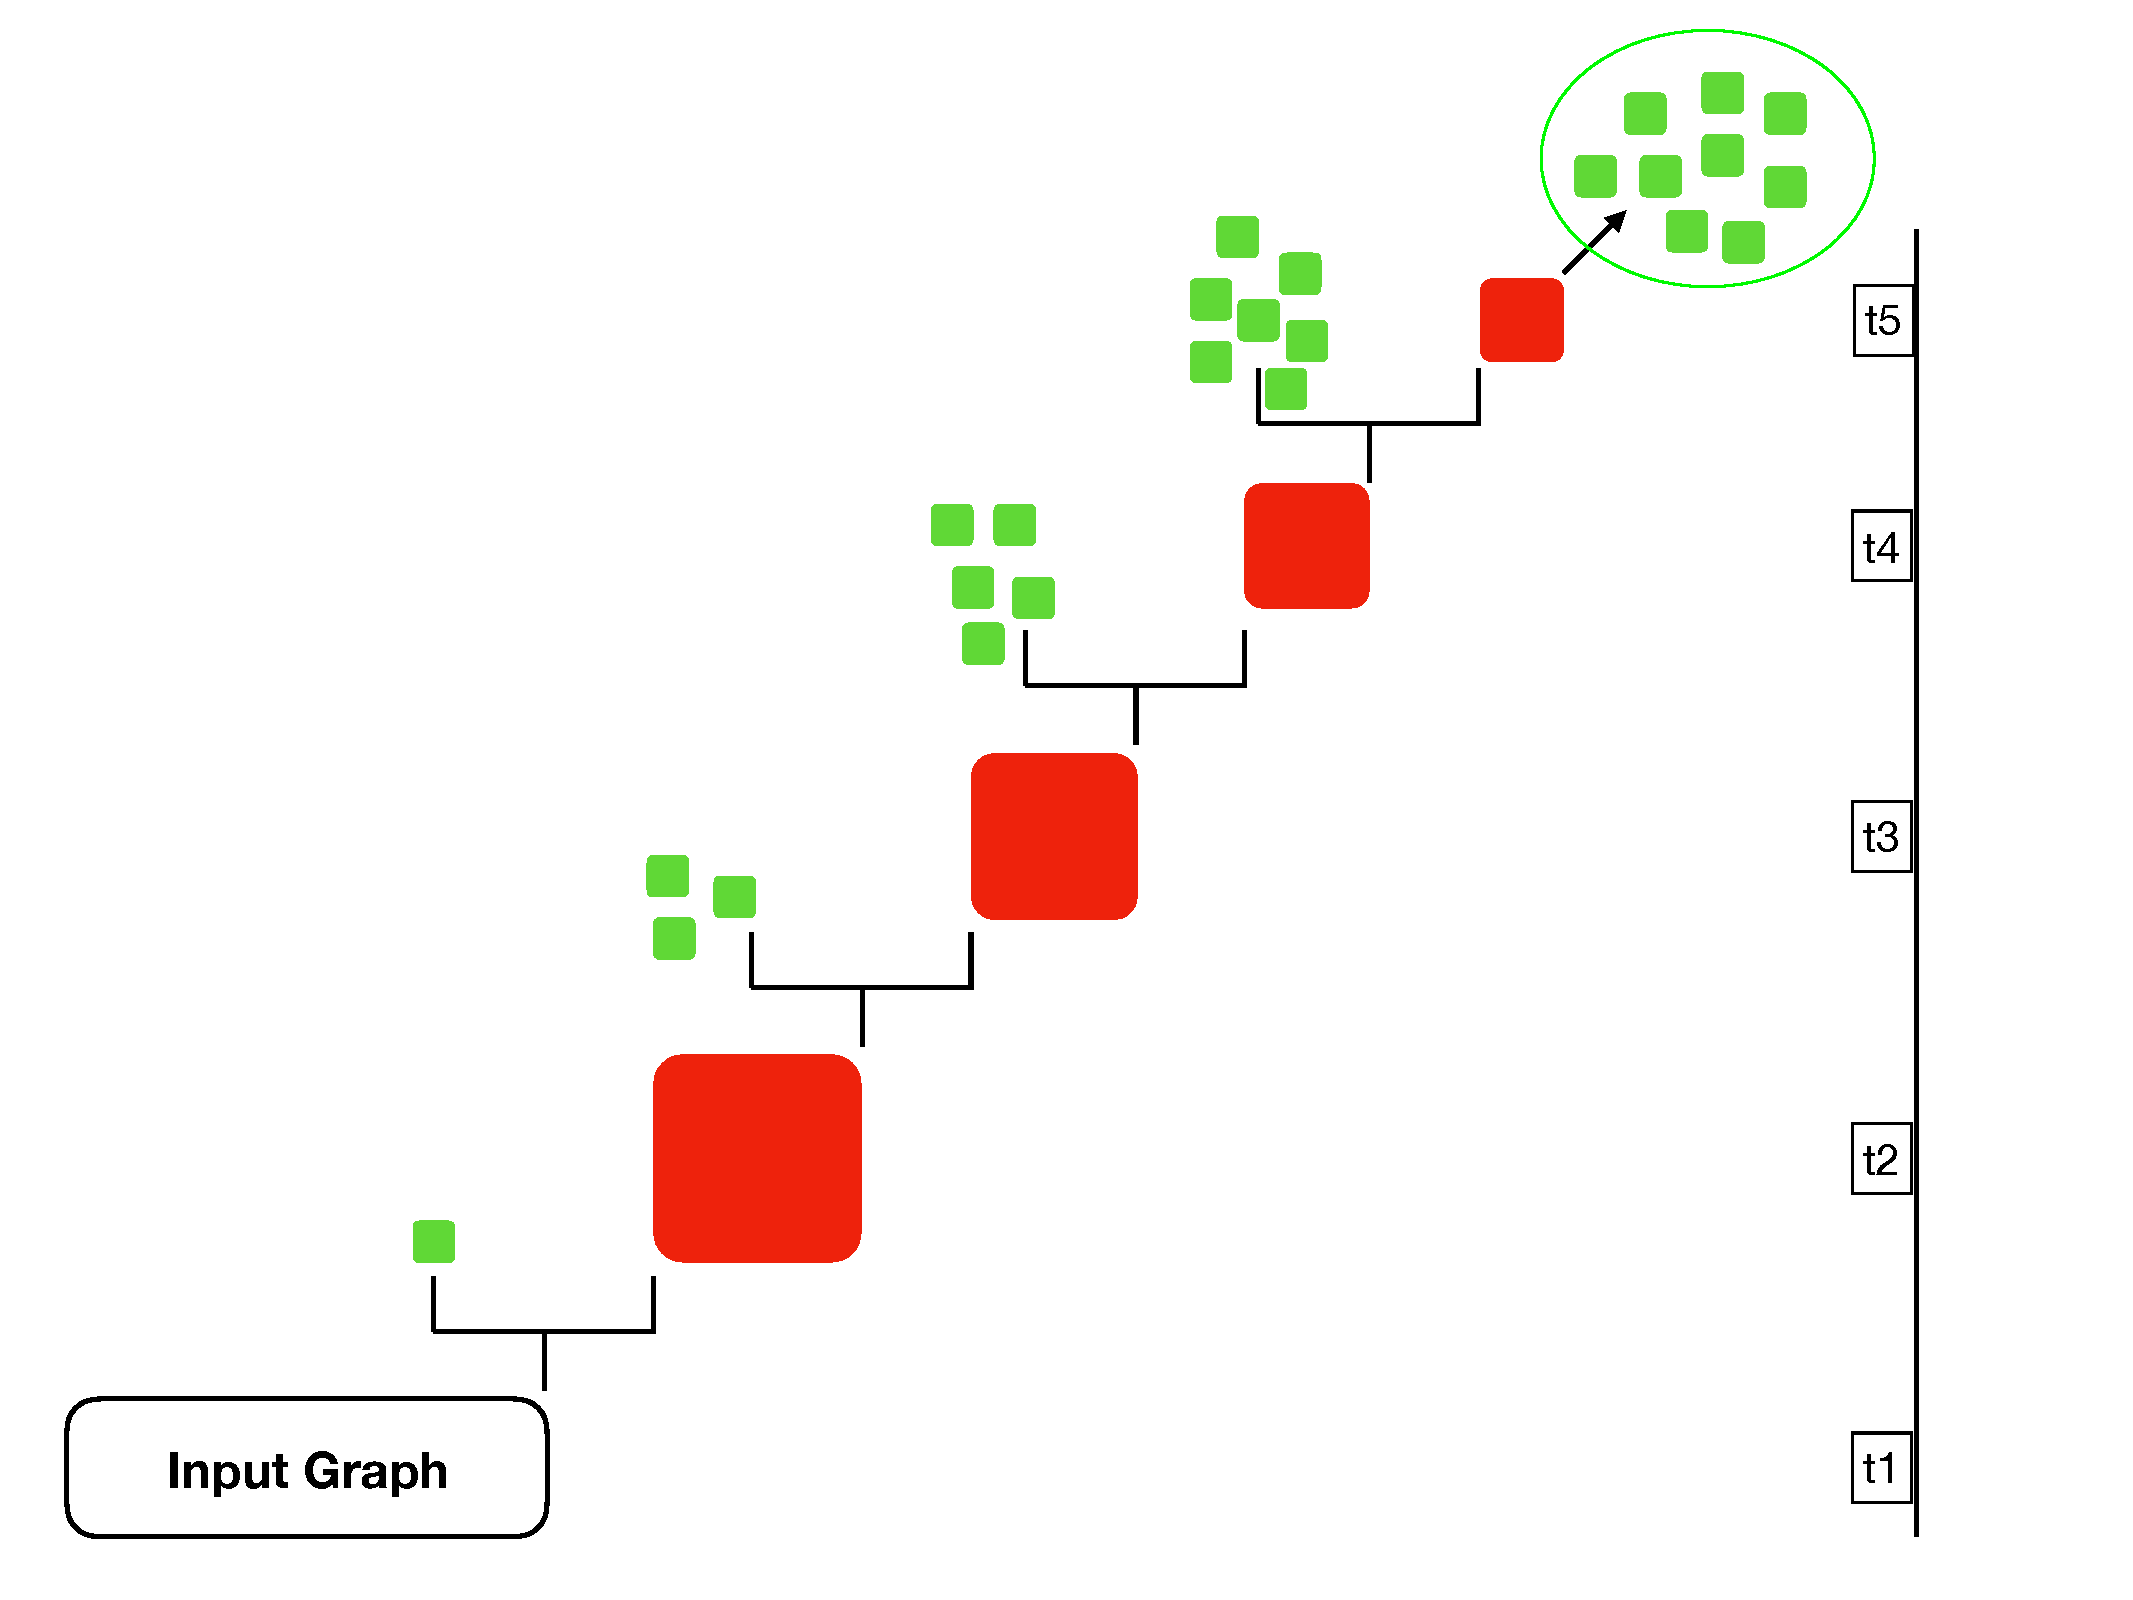
\includegraphics[scale=0.25]{vlc.pdf}
% figure caption is below the figure
\caption{Schematic representation of variable clustering protocol modified from Small and Sweeney (1985). Three parameters are specified (i) a threshold or starting level based on a quantile of normalized co-citation frequency (ii) a level increment (iii) a maximum cluster size. Input data is a set of co-cited publications with edge-weight defined by normalized co-citation frequencies. Green clusters are within the max cluster size. At the initial threshold, $t1$, a single cluster below the maximum cluster size, $mcs$ (green), along with one large cluster above it (red) are generated. As the threshold is incremented to $t2$, additional clusters of acceptable size is generated. The cascade continues to completion, which is defined by all clusters being of size less than or equal to the $mcs$. In this schematic, five rounds are adequate for the process to run to completion.}
\label{vlc_process}       % Give a unique label
\end{figure}

%\noindent
Co-citation based clustering:
\begin{enumerate}
\item Stratify by year after subsetting by COMP and restricting to article and cp only
\item Apply fractional citation counting and identify highly-cited papers
\item Calculate normalized co-citations
\item Cluster by variable clustering method of Small
\item Evaluate major co-cited pairs
\end{enumerate}

\begin{figure}[ht]
\centering
% Use the relevant command to insert your figure file.
% For example, with the graphicx package use
 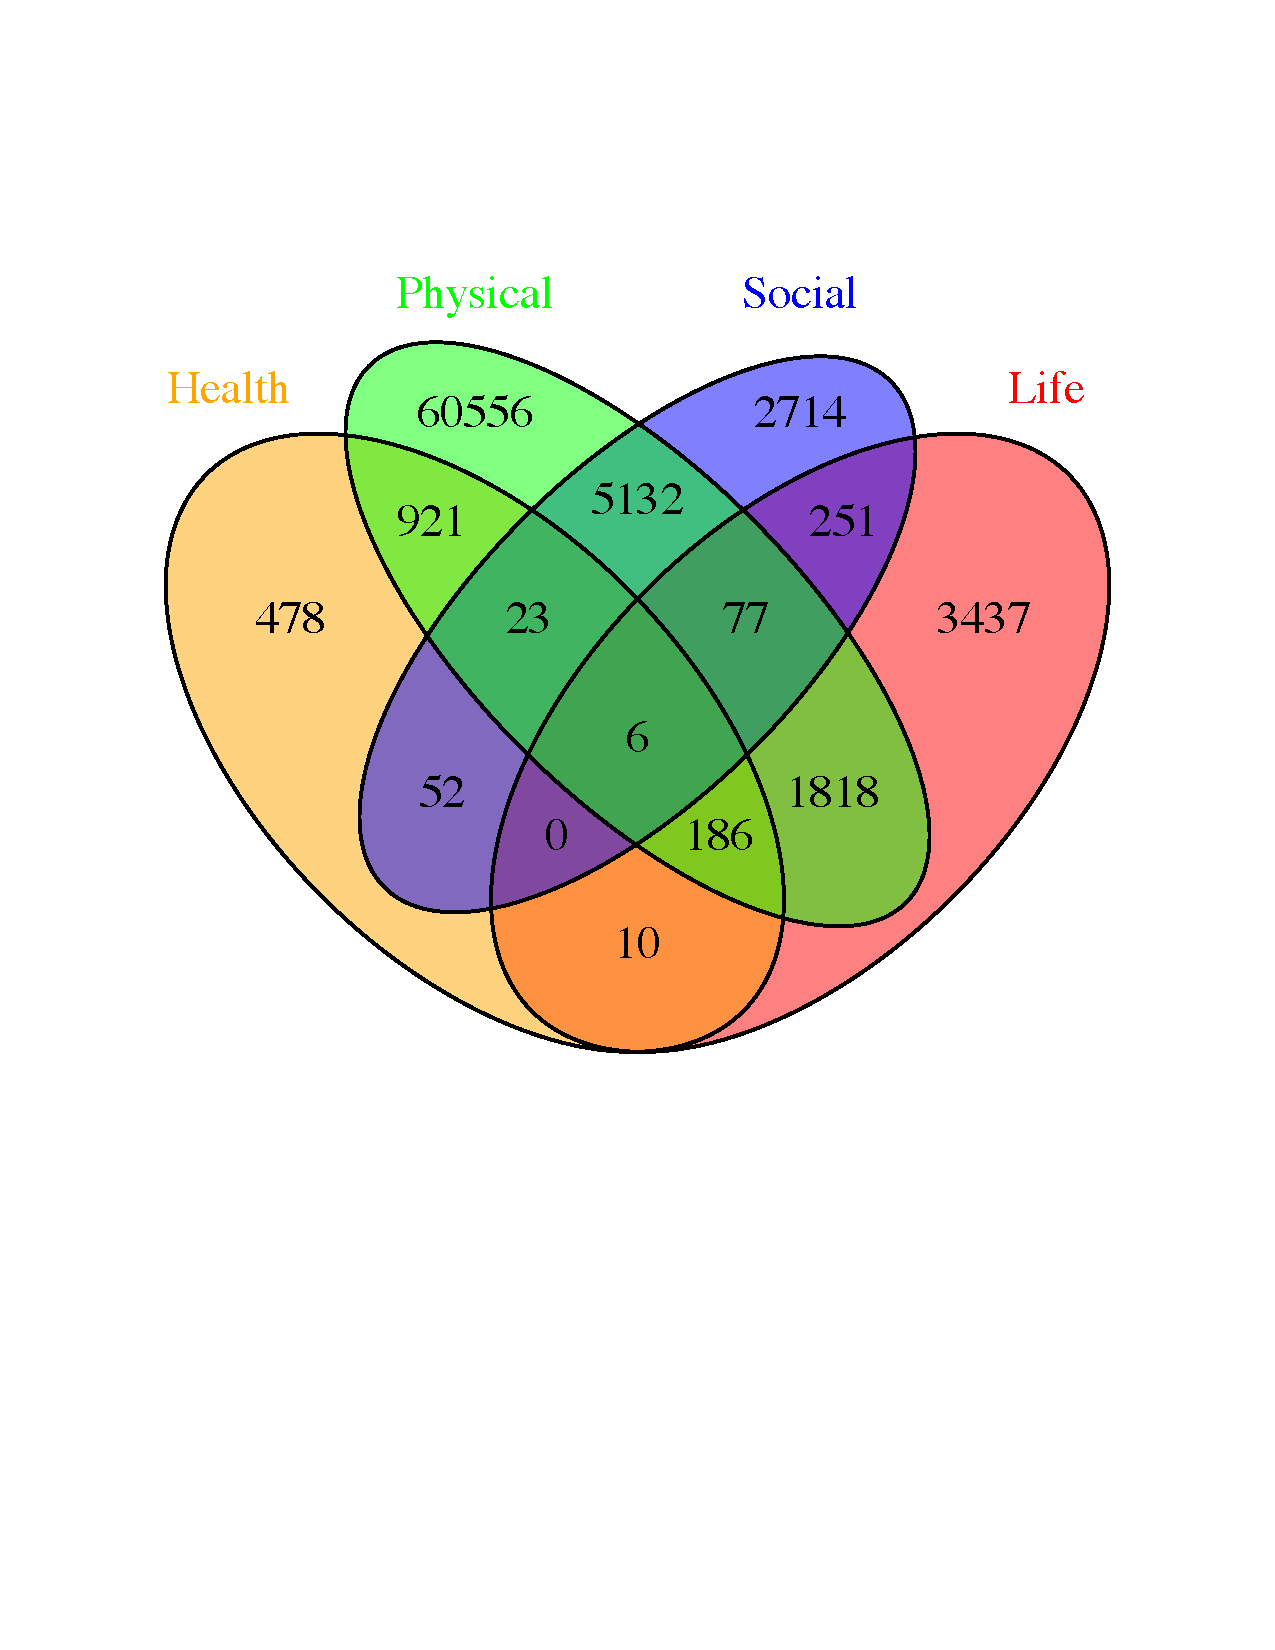
\includegraphics[scale=0.5]{cocit_venn2.pdf}
% figure caption is below the figure
\caption{High Level Disciplinary Composition of Publications in Clusters Generate by Variable Level Clustering. 84,591 nodes from were matched to the 4 subject areas, 
27 major subject areas, and 334 minor subject areas in the Scopus ASJC classification. Since 82.5\% of these nodes were assigned more to than one minor subject category, 
we assigned fractional counts for the four subject areas that summed to 1 for each article. The figure shows a four way Venn Diagram~\cite{chen_venn_2011} illustrating the 
relative frequencies of publications from the Physical Sciences, Social Sciences, Life Sciences, and Health Sciences.}
\label{fig:cocitr_venn2}       % Give a unique label
\end{figure}


\emph{need to cite Granovetter somewhere for definition of strong and weak ties that Small refers to}


%\begin{acknowledgements}
%If you'd like to thank anyone, place your comments here
%and remove the percent signs.
%\end{acknowledgements}


% Authors must disclose all relationships or interests that 
% could have direct or potential influence or impart bias on 
% the work: 
%
% \section*{Conflict of interest}
%
% The authors declare that they have no conflict of interest.


% BibTeX users please use one of
%\bibliographystyle{spbasic}      % basic style, author-year citations
\bibliographystyle{spmpsci}      % mathematics and physical sciences
%\bibliographystyle{spphys}       % APS-like style for physics
\bibliography{comp}   % name your BibTeX data base

% Non-BibTeX users please use

\clearpage



\subsection{Subsection title}
\label{sec:2}
as required. Don't forget to give each section
and subsection a unique label.
\paragraph{Paragraph headings} Use paragraph headings as needed.
\begin{equation}
a^2+b^2=c^2
\end{equation}

% For one-column wide figures use
\begin{figure}
% Use the relevant command to insert your figure file.
% For example, with the graphicx package use
  \includegraphics{example.eps}
% figure caption is below the figure
\caption{Please write your figure caption here}
\label{fig:1}       % Give a unique label
\end{figure}
%
% For two-column wide figures use
\begin{figure*}
% Use the relevant command to insert your figure file.
% For example, with the graphicx package use
  \includegraphics[width=0.75\textwidth]{example.eps}
% figure caption is below the figure
\caption{Please write your figure caption here}
\label{fig:2}       % Give a unique label
\end{figure*}
%
% For tables use


\section{Garbage}

Cite Alan Porter on expanding universe versus myopic focus. Cite Traag, Waltman, Lariviere papers. Peter Sjögårde and Per Ahlgren, Loet Leydesdorff, Caroline S. Wagner and Lutz Bornmann, Discontinuities in citation relations among journals: self-organized criticality as a model of scientific revolutions and change, Scientometrics, 10.1007/s11192-018-2734-6, 116, 1, (623-644), (2018). Antonio Perianes-Rodriguez and Javier Ruiz-Castillo, A comparison of the Web of Science and publication-level classification systems of science, Journal of Informetrics, 10.1016/j.joi.2016.10.007, 11, 1, (32-45), (2017). Qi Wang and Ludo Waltman, Large-scale analysis of the accuracy of the journal classification systems of Web of Science and Scopus, Journal of Informetrics, 10.1016/j.joi.2016.02.003, 10, 2, (347-364), (2016). Henry Small, Kevin W. Boyack and Richard Klavans, Identifying emerging topics in science and technology, 
Crossref

\textcolor{blue}{George, the rest needs to go into methods}


\paragraph{Overall strategy}

Here we describe the overall strategy used for the two clustering methods.\\

\emph{misc stuff:  In using the term inform, we are mindful of (i) Greenhalgh (ii) Sarewitz and Pielke. I think that I want to cite these two without really knowing how. Greenhalgh for the limitations of positivism. Sarewitz for the limitations of allowing science to do whatever it wants to. I'd also like to see some text about (i) limited funding resources (ii) efficient use of existing resources (iiii) informing policy at multiple levels -- all directed at justifying our study. I'm not sure where to put it though. CS can also be an excellent model system for studying interdisciplinarity cite Porter and colleagues in a study on measuring interdisciplinarity~\cite{porter_measuring_2007} observe that 'The discrepancies between disciplinary roots and research realities loom large', a reference to the challenges associated with knowledge diffusing across researchers who tend to be focused in their own areas. This concern may be especially relevant for computer science given the ubiquity of computing today and limited public funding for research. Maybe squeeze in Tandy's NAS report on interdisciplinarity. I should ping Ohid Yaqub about this too- science policy is his area.}


\noindent
 Spectral clustering:
\begin{enumerate}
\item Subset Scopus by COMP
\item Match COMP to DBLP at high stringency -> reduced number of scps
 \item Harvest cited references  from Scopus
 \item Cluster articles by direct citation using Graclus to a number that meets simple optimality criteria and does not impose cognitive challenges
 \item Reconcile cluster contents to journal classification for the purpose of referencing
 \item Infer inter-cluster relationships using direct citations, co-citations, and bibliographic coupling
\end{enumerate}

\end{document}
% end of file template.tex

